% Kompiuterijos katedros ir kibernetinio saugumo laboratorijos šablonas
% Template of Department of Computer Science II or cybersecurity laboratory
% Versija 1.4 2024 m. sausi [ March, 2015]
% comments/bug fixes send to template authors: Linas Bukauskas or Agnė Brilingaitė
\documentclass[a4paper,12pt,fleqn]{article}
\usepackage[unicode,colorlinks=false]{hyperref}


\usepackage[utf8x]{inputenc}
%

\usepackage[L7x]{fontenc}
\usepackage{times}
\usepackage{ucs}
%\usepackage{microtype}
%\DisableLigatures{encoding = *, family = *}
 %package to switch the language
\usepackage{etoolbox}

  %set up of the page margins
\usepackage[top=2cm, bottom=2cm, left=3cm, right=1.5cm]{geometry}

 %1.1 line spacing
\linespread{1.1}


  %page numbering at the right side
\usepackage{fancyhdr}
\pagestyle{fancyplain}
\fancyhf{}
\renewcommand{\headrulewidth}{0pt} 
\fancyhfoffset[RO]{0cm}

  %to number at the bottom (exchange lines to number at the top)
\rfoot{\thepage}
  %\rhead{\thepage} %

% \usepackage[usenames,dvipsnames]{pstricks}
\urlstyle{same}
\hypersetup{
%  citecolor=Blue,
%  linkcolor=Blue,
%  urlcolor=Blue
pdfborder={0 0 0 }
}

 %for includegraphics
\usepackage{graphicx}

\usepackage[toc,page]{appendix}


\usepackage{caption}

 %for source codes
\usepackage{listings}
\lstset{commentstyle=\color{red},xleftmargin=10pt, framexleftmargin=6pt, numbersep=1mm, frame=single, numbers=left,numberstyle=\footnotesize,extendedchars=\true, inputencoding=utf8x,basicstyle=\footnotesize,extendedchars=true,
 keywordstyle=\color{black}\bfseries, breaklines=true, breakautoindent=true,framesep=8pt,linewidth=0.95\textwidth
}

 %for algorithms
\usepackage{algorithm}
\usepackage{algorithmic}
 %instead of the above two packages we can use algorithms2e
 %\usepackage[boxed,linesnumbered,vlined,slide]{algorithm2e}

 %special symbols
\usepackage{amsfonts}
%\usepackage{amssymb} %redundant
\usepackage{amsmath}

 %for theorem like environments
\usepackage{amsthm}

 \usepackage{datetime}
 \renewcommand{\dateseparator}{--}


% SI system units
\usepackage{siunitx}
\sisetup{detect-all}
% Problem with fonts \SI{x.xx}{\micro\metre}, solved with updmap-sys --enable Map=utm.map
\renewcommand{\sfdefault}{uhv}
%\renewcommand{\rmdefault}{utm}  %commented due to text missformating
\usepackage{stix}
\renewcommand{\ttdefault}{ucr}

% List management (itemize, etc.)
\usepackage{enumitem}

\newcommand*{\urlw}[1]{\href{#1}%
            {\nolinkurl{#1}}}

\numberwithin{equation}{section}


%%%%%%%%%%% lino įdėta
%
\usepackage{pifont,mdframed}

\newenvironment{warning}
  {\par\begin{mdframed}[linewidth=2pt,linecolor=red]%
    \begin{list}{}{\leftmargin=1cm
                   \labelwidth=\leftmargin}\item[\Large\ding{43}]}
  {\end{list}\end{mdframed}\par}
  

\newtoggle{inLithuanian}
 %If the report is in Lithuanian, it is set to true; otherwise, change to false
\settoggle{inLithuanian}{false}

%create file preface.tex for the preface text
%if preface is needed set to true
\newtoggle{needPreface}
\settoggle{needPreface}{false}

\newtoggle{signaturesOnTitlePage}
\settoggle{signaturesOnTitlePage}{false}


\theoremstyle{definition}
\newtheorem{definition}{\keyWordDefinition}
\newtheorem{example}{\keyWordExample}
\def\QED{\unskip\nobreak\hfill\kern5pt$\Box$}

\iftoggle{inLithuanian}{
%\usepackage[L7x]{fontenc}
\usepackage[english,lithuanian]{babel}

\newcommand{\todayiso}{\the\year \dateseparator \twodigit\month \dateseparator \twodigit\day}


\renewcommand{\today}{\number\year\space m. \space \ifcase\month\or
  sausio\or vasario\or kovo\or balandžio\or gegužės\or birželio\or
  liepos\or rugpjūčio\or rugsėjo\or spalio\or lapkričio\or
  gruodžio\fi
  \space\number\day\space d.}


 \usepackage{tocloft}
 \renewcommand\cftsecaftersnum{.} 
 \renewcommand\cftsubsecaftersnum{.} 
 \renewcommand\cftsubsubsecaftersnum{.}

 \usepackage{VUMIFKK}

 \DeclareCaptionLabelFormat{captionlt}{#2 #1}
   %smth is not fine with algorithms 
 \DeclareCaptionLabelFormat{captionltalg}{#2 #1 algoritmas}

 \usepackage{indentfirst}
 \renewcommand{\appendixtocname}{Priedai}
 \renewcommand{\appendixpagename}{Priedai}
 \renewcommand{\contentsname}{Turinys} 

 \renewcommand{\lstlistingname}{išeities kodas}
 \renewcommand{\figurename}{pav}
 \renewcommand{\tablename}{lentelė}


 \captionsetup*[lstlisting]{   
 labelsep=period,labelformat=captionlt
 }
 \captionsetup*[figure]{   
% labelsep=period,
 labelsep=space, %babel redefines pav to pav.
 labelformat=captionlt
 }
 \captionsetup*[table]{   
  labelsep=period,
  labelformat=captionlt
 }
 \renewcommand{\algorithmicrequire}{\textbf{Įvestis:}}
 \renewcommand{\algorithmicensure}{\textbf{Išvestis:}}

 \captionsetup*[algorithm]{   
 labelsep=period,labelformat=captionltalg
 }

\renewcommand{\thmhead}[3]{#2 #1#3}

}
{
%\usepackage[OT1,T1]{fontenc}
%\usepackage[L7x]{fontenc}



\usepackage[english]{babel}
\newcommand{\todayiso}{\twodigit\month \dateseparator \twodigit\day \dateseparator \the\year}
 \captionsetup*[algorithm]{   
 labelsep=period
 }
\captionsetup*[lstlisting]{   
 labelsep=period
 }
 \captionsetup*[figure]{   
 labelsep=period
 }
 \captionsetup*[table]{   
 labelsep=period
 }


}

%some kywords
 \def\keywordAbstract{\iftoggle{inLithuanian}{Santrauka}{Abstract}}
 \def\keywordAbstractOther{\iftoggle{inLithuanian}{Summary}{Santrauka}}
 \def\keyWordIntroduction{\iftoggle{inLithuanian}{Įvadas}{Introduction}}
 \def\keyWordConclusions{\iftoggle{inLithuanian}{Išvados ir rekomendacijos}{Conclusions and Recommendations}}

 \def\keyWordPreface{\iftoggle{inLithuanian}{Pratarmė}{Preface}}
 \def\keyWordAppendice{\iftoggle{inLithuanian}{Priedas}{Appendix}}
 \def\keyWordSignature{\iftoggle{inLithuanian}{parašas}{signature}}
 \def\keyWordDefinition{\iftoggle{inLithuanian}{apibrėžimas}{Definition}}
 \def\keyWordExample{\iftoggle{inLithuanian}{pavyzdys}{Example}}

\newcommand{\bothabstracts}[3]{
\setcounter{secnumdepth}{0}
\newpage
\hspace{2cm}
{\centering{\section{\keywordAbstract}}}

#1
\newpage
\hspace{2cm}
{\centering \section{\keywordAbstractOther}}

\begin{center}{\textbf{#2} }\end{center}

 #3
\setcounter{secnumdepth}{3}
}

 %non-numbered sections: #1 param: for labeling sec:#1, #2 -section title
\newcommand{\sectionWithoutNumber}[2]{\newpage
%\hspace{2cm}
\section*{#1}
\label{sec:#2}
\addcontentsline{toc}{section}{\nameref{sec:#2}}%{#3}
 }



\newcommand{\referenceSources}[1]{
\newpage
\cleardoublepage
\phantomsection
\iftoggle{inLithuanian}{
 \renewcommand{\refname}{Literatūros šaltiniai}

 \addcontentsline{toc}{section}{Literatūros šaltiniai}
 \markboth{\refname}{Literatūros šaltiniai}
 }
{

\addcontentsline{toc}{section}{References}
\markboth{References}{References}
}

\bibliographystyle{plain}
\bibliography{#1}
}



 \newcommand\authorsignature[1]{
\begin{flushright}
 \begin{minipage}[b]{0.45\textwidth}
  \centering
  \rule{\textwidth}{0.5pt}\\
   #1
  \end{minipage}
\end{flushright}
 }




 \newcommand\authorsignatures[5]{%
   \vspace{1cm}
   \authorsignature{#1}
   \ifstrequal{#2}{}{}{\vspace{0.3cm}
     \authorsignature{#2}
     \ifstrequal{#3}{}{}{\vspace{0.3cm}
      \authorsignature{#3}
      \ifstrequal{#4}{}{}{\vspace{0.3cm}
        \authorsignature{#4}
        \ifstrequal{#5}{}{}{\vspace{0.3cm}
         \authorsignature{#5}       
        }
      }
    }
} 
}

\newcommand{\authortitle}{
\iftoggle{signaturesOnTitlePage}{
\tiny{\keyWordSignature}
}{}
}

\newcommand{\depttitlepage}[8]
{
\thispagestyle{empty}
\begin{center}


\includegraphics[width=2cm]{jb_VU_zenklas}

%\vspace{-1cm}

\iftoggle{inLithuanian}
{ 
  VILNIAUS UNIVERSITETAS\\
  MATEMATIKOS IR INFORMATIKOS FAKULTETAS\\
  INFORMATIKOS INSTITUTAS\\
  <<KOMPIUTERINIO IR DUOMENŲ MODELIAVIMO KATEDRA>> ARBA \\ <<KIBERNETINIO SAUGUMO LABORATORIJA>>
}
{
  VILNIUS UNIVERSITY \\
  FACULTY OF MATHEMATICS AND INFORMATICS \\
  INSTITUTE OF COMPUTER SCIENCE\\
  <<DEPARTMENT OF COMPUTATIONAL AND DATA MODELING>> OR \\ <<CYBERSECURITY LABORATORY>>
}

\vspace{5cm}

#1\\
\vspace{0.5cm}
\textbf{\Large #2}
\end{center}

\vspace{5cm}


\hspace{0.5\textwidth}
\begin{minipage}{0.4\textwidth}
 \begin{flushleft} 
\iftoggle{inLithuanian}
{
 \ifstrequal{#3}{}{}{Atliko:\\[5pt]}
}
{
\ifstrequal{#3}{}{}{Done by:\\[5pt]}
}
%\noindent
\begin{tabular}{@{}lr}%\setlength\tabcolsep{0pt}
\ifstrequal{#3}{}{}{#3&\hspace{2cm}\authortitle\\[5pt]}
\ifstrequal{#4}{}{}{#4&\authortitle\\[5pt]}
\ifstrequal{#5}{}{}{#5&\authortitle\\[5pt]}
\ifstrequal{#6}{}{}{#6&\authortitle\\[5pt]}
\ifstrequal{#7}{}{}{#7&\authortitle\\}
\end{tabular}

\end{flushleft}

\end{minipage}

\vspace{0.5cm}
\hspace{0.5\textwidth}
\begin{minipage}{0.4\textwidth}
 \begin{flushleft} 

\ifstrequal{#8}{}{}
{

\iftoggle{inLithuanian}
{
Vadovas:
}
{
Supervisor:
}

#8

}

\end{flushleft}

\end{minipage}


\vfill

\begin{center}
Vilnius\\
\the\year
\end{center}

\iftoggle{needPreface}{
 \sectionWithoutNumber{\keyWordPreface}{preface}
Pratarmės (Preface) informacija


\iftoggle{inLithuanian}
{
\vspace{\baselineskip}\hfill
\today
}
{
 \vspace{\baselineskip}\hfill \today
}

 \vspace{5cm}

\iftoggle{signaturesOnTitlePage}{}
{
\authorsignatures{#3}{#4}{#5}{#6}{#7}
}
}{}
\newpage
}


\begin{document}
 % #1 -report type, #2 - title, #3-7 students, #8 - supervisor
 \depttitlepage{Course project no. 2}{Fourier filter\\{\small Based on Cooley-Tuckey algorithm}}{Kazimieras Vitkus}{}{}{}{}{Prof. Tadas Meskauskas}

\tableofcontents
\newpage

\section{Introduction}
\hspace{1 em}In the realm of digital signal processing, the Fast Fourier Transform (FFT) and its inverse (IFFT) are pivotal algorithms that enable efficient computation of the Discrete Fourier Transform (DFT) and its inverse (IDFT). These mathematical tools transform time-domain signals into their frequency-domain representations and vice versa, offering profound insights into the frequency components of signals. Implementing these transformations from scratch not only deepens the understanding of their mechanics but also highlights the computational optimizations that FFT introduces over the traditional DFT.

This report details the implementation of FFT, IFFT, DFT, and IDFT algorithms from the ground up. We will explore how these algorithms can be utilized for high-pass and low-pass filtering, allowing us to isolate and analyze specific frequency components within sound signals. By filtering and examining these signals, we gain a better understanding of the underlying structures and characteristics of different audio samples.

\section{Algorithm implementation}

\subsection{Discrete Fourier Transform (DFT)}

\hspace{1 em}The Discrete Fourier Transform (DFT) is a mathematical operation that transforms a finite sequence of equally spaced samples of a function into a sequence of complex numbers. The DFT is defined by the formula:

\begin{equation}
    C_k = \sum_{j=0}^{N-1} f_j \cdot e^{-\frac{2\pi i}{N}kn}
\end{equation}
  
  where $f_j$ is the input signal, $C_k$ is the output signal, and $N$ is the number of samples in the input signal. The DFT algorithm computes the frequency components of the input signal by summing the product of each sample with a complex exponential function.
  In my implementation, I used the following Python code to calculate the DFT of an input signal:

\begin{lstlisting}[language=Python]
def dft(signal):
  
  N = len(signal)
  
  C_k = np.zeros(N, dtype=np.complex_)
  
  for k in range(N):
      
      for n in range(N):
          C_k[k] += signal[n] * np.exp(-2j * np.pi * k * n / N)
      
      C_k[k] /= N
  return C_k
\end{lstlisting}

\newpage
for the inverse DFT, we can use the following code:
\begin{lstlisting}[language=Python]
def idft(signal):
  
  N = len(signal)
  
  f_j = np.zeros(N, dtype=np.complex_)
  
  for j in range(N):
      
      for k in range(N):
          f_j[j] += signal[k] * np.exp(2j * np.pi * k * j / N)
      
  return f_j
\end{lstlisting}

\subsection{Fast Fourier Transform (FFT)}

\hspace{1 em}The Fast Fourier Transform (FFT) is an algorithm that computes the Discrete Fourier Transform (DFT) of a sequence of complex numbers. The FFT is an optimized version of the DFT that reduces the number of arithmetic operations required to compute the DFT from $O(N^2)$ to $O(N \log N)$. The Cooley-Tukey algorithm is a popular implementation of the FFT that recursively divides the input sequence into smaller sub-sequences and combines the results to compute the DFT.

In my implementation, I used the following Python code to calculate the FFT of an input signal:
\begin{lstlisting}[language=Python]
def fft(signal):
  N = len(signal)
  
  if N <= 1:
      return signal
      
  fft_even = fft(signal[::2])
  fft_odd = fft(signal[1::2])
  
  k = np.arange(N // 2)
  W_n_k = np.exp(-2j * np.pi * k / N)
  
  A_k = fft_even
  B_k = fft_odd * W_n_k
  
  C_k = np.zeros(N, dtype=np.complex_)
  C_k[:N // 2] = A_k + B_k
  C_k[N // 2:] = A_k - B_k
  
  return C_k 
  
\end{lstlisting}
\newpage
For the inverse FFT, we can use the following code:

\begin{lstlisting}[language=Python]
def ifft(signal):
N = len(signal)

if N <= 1:
    return signal

ifft_even = ifft(signal[::2])
ifft_odd = ifft(signal[1::2])

k = np.arange(N // 2)
W_n_k = np.exp(2j * np.pi * k / N)

A_k = ifft_even
B_k = ifft_odd * W_n_k

f_j = np.zeros(N, dtype=np.complex_)
f_j[:N // 2] = A_k + B_k
f_j[N // 2:] = A_k - B_k

return f_j / N




\end{lstlisting}


\section{Analysis of algorithms and implementation}

\subsection{Comparison of DFT and FFT}

\hspace{1 em}In theory and practice, the Fast Fourier Transform (FFT) is significantly 
faster than the Discrete Fourier Transform (DFT) for computing the frequency components 
of a signal. The FFT algorithm reduces the number of arithmetic operations required 
to compute the DFT from $O(N^2)$ to $O(N \log N)$, making it much more efficient for 
large input signals. For the example of comparison, signal was generated using numpy
random function with length varying from $2^2$ to $2^7$.

\begin{figure}[H]
    \centering
    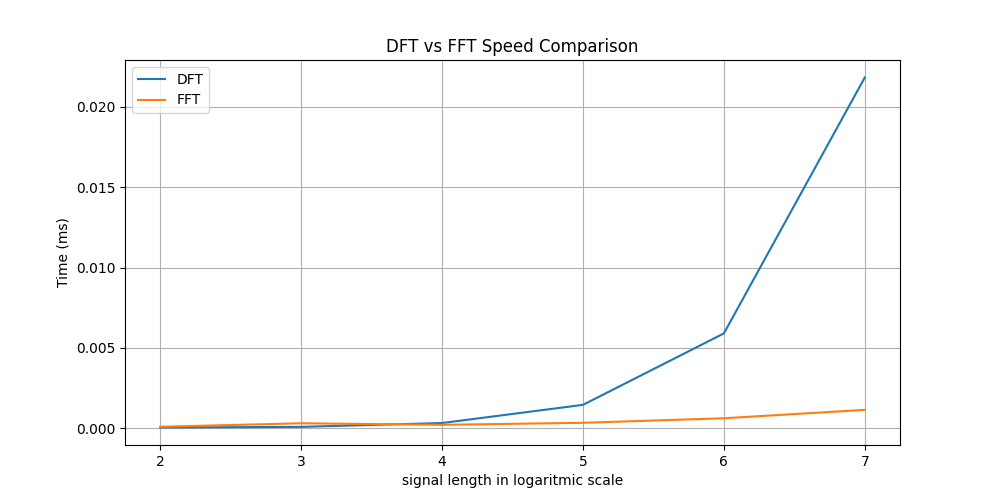
\includegraphics[width=1\textwidth]{dft_vs_fft.png}
    \caption{Comparison of computation time between DFT and FFT}
    \label{fig:fft_vs_dft}
\end{figure}

As can be seen in figure \ref{fig:fft_vs_dft}, the FFT algorithm is significantly faster. 
The trend line for DFT seems to be increasing exponentially, while the FFT trend line
is almost linear. This demonstrates the computational efficiency of the FFT algorithm
compared to the DFT algorithm. However, the chart may vary depending on the length of 
the input signal used for comparison.

\subsection{Comparison of FFT from scratch and numpy FFT}

\hspace{1 em}The numpy library provides a built-in FFT function that is highly optimized
and efficient for computing the Discrete Fourier Transform (DFT) of a signal. In this
section, we compare the performance of the FFT algorithm implemented from scratch with
the numpy FFT function. The signal was generated using numpy random function with length
varying from $2^2$ to $2^{16}$.

\begin{figure}[H]
    \centering
    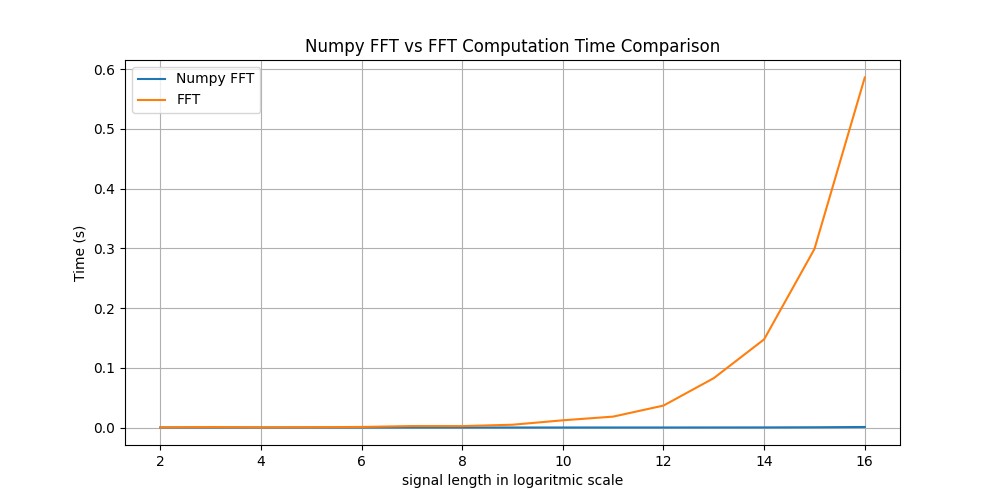
\includegraphics[width=1\textwidth]{np_fft_fft.png}
    \caption{Comparison of computation time between FFT from scratch and numpy FFT}
    \label{fig:fft_vs_numpy_fft}
\end{figure}

As can be seen in figure \ref{fig:fft_vs_numpy_fft}, the numpy FFT function is significantly
faster than the FFT algorithm implemented from scratch. After certain length of the input, implementation
from scratch seems to differ exponentially in computation times. It means, implementation quality is
suboptimal and needs to be improved.

\subsection{Fitting requirements for algorithm reduces performance}

\hspace{1 em} One of requirements for signal that needs to be processed with FFT - 
it's length must be a power of 2. One of the provided solutions - zero padding, which
means adding zeros to the end of the signal to make it's length a power of 2. However,
this solution may reduce the performance of the FFT algorithm. In this section, we compare
the performance of the FFT algorithm with and without zero padding. The signal was generated
using numpy random function with length varying from $2^2$ to $2^{16}$ and for comparison, one signal has
$0$ appended to invoke zero padding function.

\begin{figure}[H]
    \centering
    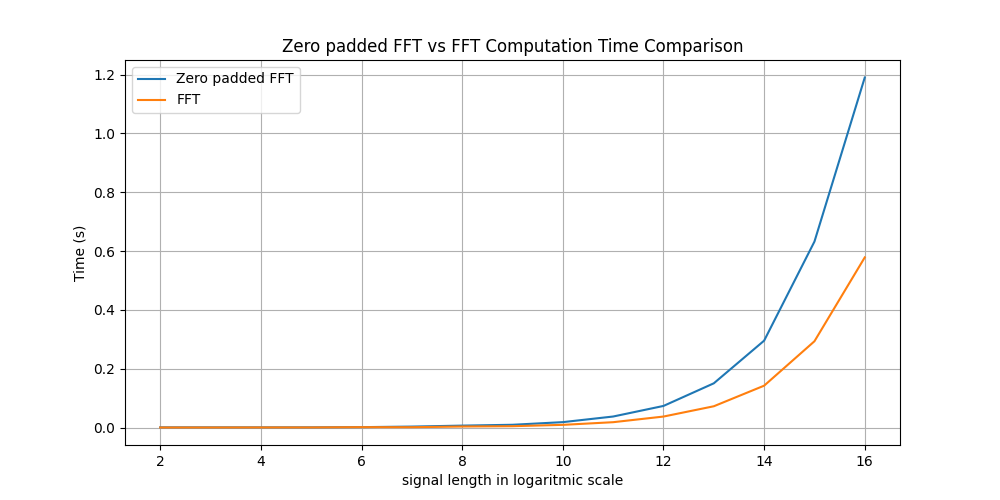
\includegraphics[width=1\textwidth]{zerop_fft_fft.png}
    \caption{Comparison of computation time between FFT with and without zero padding}
    \label{fig:zero_padding}
\end{figure}

As can be seen in figure \ref{fig:zero_padding}, the signal, that invokes zero padding, takes 
more time to compute the FFT algorithm. The relation between computation times, is that if zero padding
was invoked, the computation equals to the computation time of signal with length $2^{k+1}$.


\section{Audio signal filtering}

\hspace{1 em} For the demonstration of the Fourier filter, we will use a sample audio signal.
The signal was downloaded from the following website: \url{https://freesound.org/people/InspectorJ/sounds/412067/}.

The signal in an unprocessed form is presented in figure \ref{fig:unprocessed_signal}. 
It is based on framerate of 44100 Hz and has 2 channels. The signal consists of 115327 frames and is of 2.5 seconds duration.
The signal is not compressed and saved in the wave (WAV) format.
\begin{figure}[H]
    \centering
    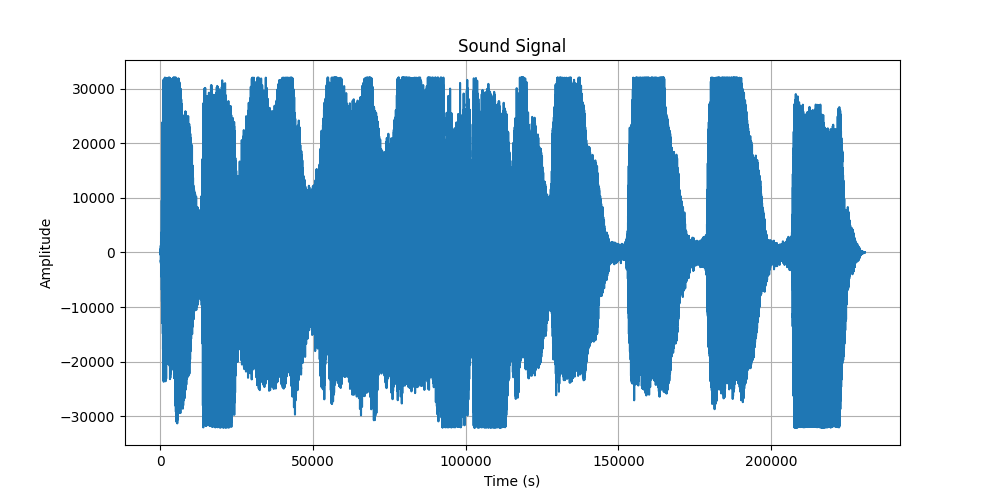
\includegraphics[width=1\textwidth]{unprocessed_signal.png}
    \caption{Unprocessed audio signal}
    \label{fig:unprocessed_signal}
\end{figure}

The power spectrum of the signal is presented in figure \ref{fig:power_spectrum}. The power spectrum
shows the frequency components of the signal. The x-axis represents the frequency in Hz, while the y-axis
represents the power of the signal at each frequency in decibels (logarithmic scale). The power spectrum provides insights into the frequency
components of the signal and can be used to identify specific frequency ranges for filtering.


\begin{figure}[H]
    \centering
    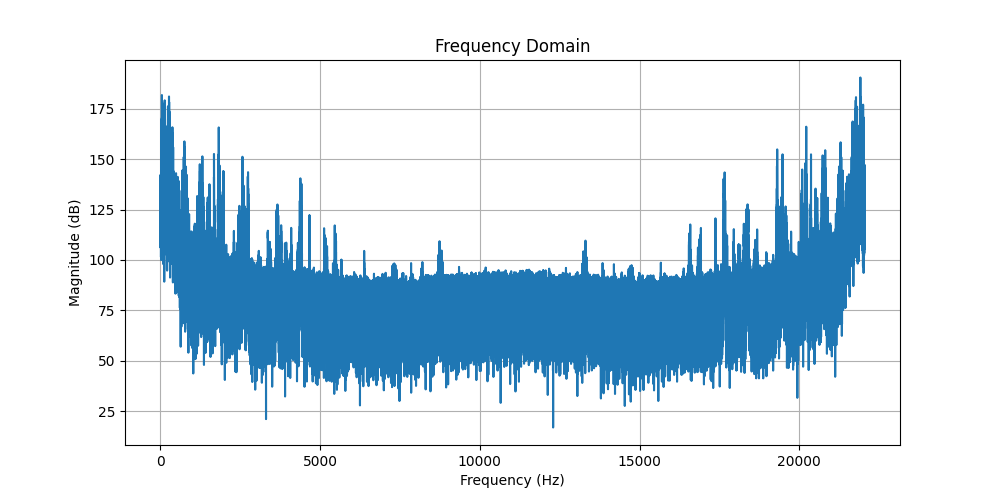
\includegraphics[width=0.8\textwidth]{frequency_domain.png}
    \caption{Power spectrum of the audio signal}
    \label{fig:power_spectrum}
\end{figure}

Also signal when transformed to frequency domain, can also be plotted in histgram form. 
The histogram of the signal is presented in figure \ref{fig:histogram}. The 
histogram shows the distribution of the signal values in the frequency domain. 
The x-axis represents the frequency bins, while the y-axis represents the number of
 occurrences of each frequency bin. The histogram provides insights into the distribution
  of frequency components in the signal and can be used to identify specific frequency 
  ranges for filtering.
  \begin{figure}[H]
    \centering
    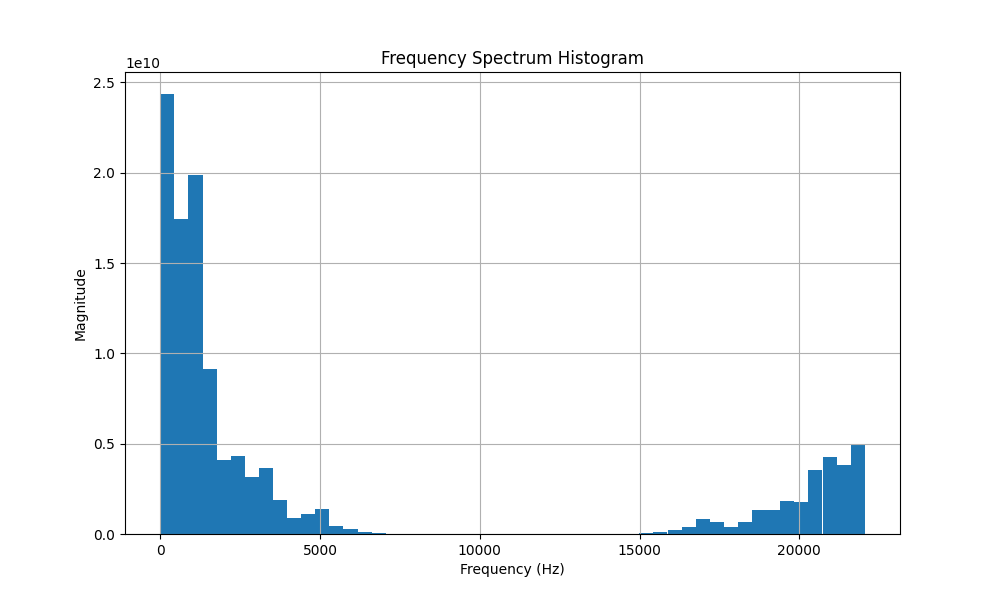
\includegraphics[width=0.8\textwidth]{original_spectrum_histogram.png}
    \caption{Signal in frequency domain and histogram}
    \label{fig:histogram}
\end{figure}
\subsection{High-pass filtering}

\hspace{1 em} High-pass filtering is a signal processing technique that allows high-frequency components of a signal to pass through while attenuating low-frequency components. In this section, we will implement a high-pass filter using the Fourier transform and apply it to the audio signal.
In the scope of this task, prebuilt function was made, that takes in signal and frequency that is The
threshold frequency for the high-pass filter. The function returns the filtered signal.



\begin{figure}[H]
    \centering
    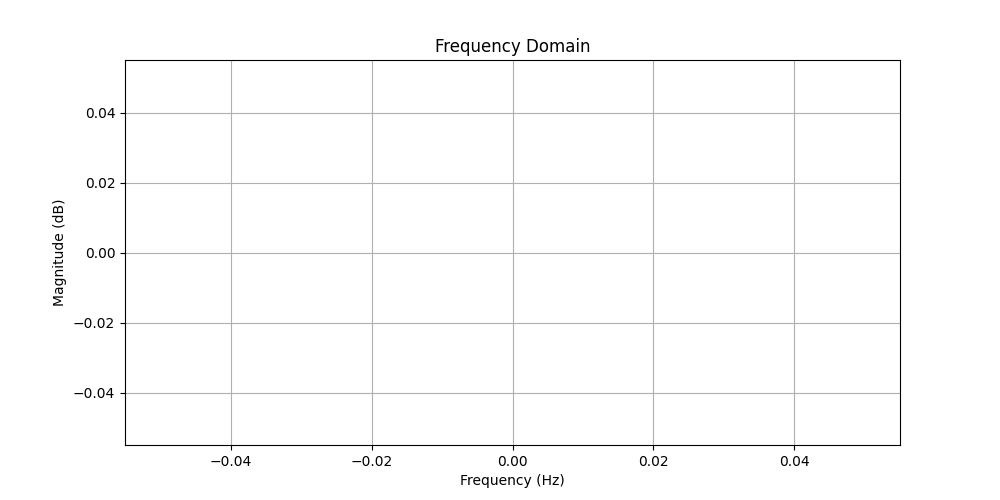
\includegraphics[width=1\textwidth]{high_pass_filter.png}
    \caption{High-pass filtered audio signal}
    \label{fig:high_pass_filter}
\end{figure}
\begin{figure}[H]
    \centering
    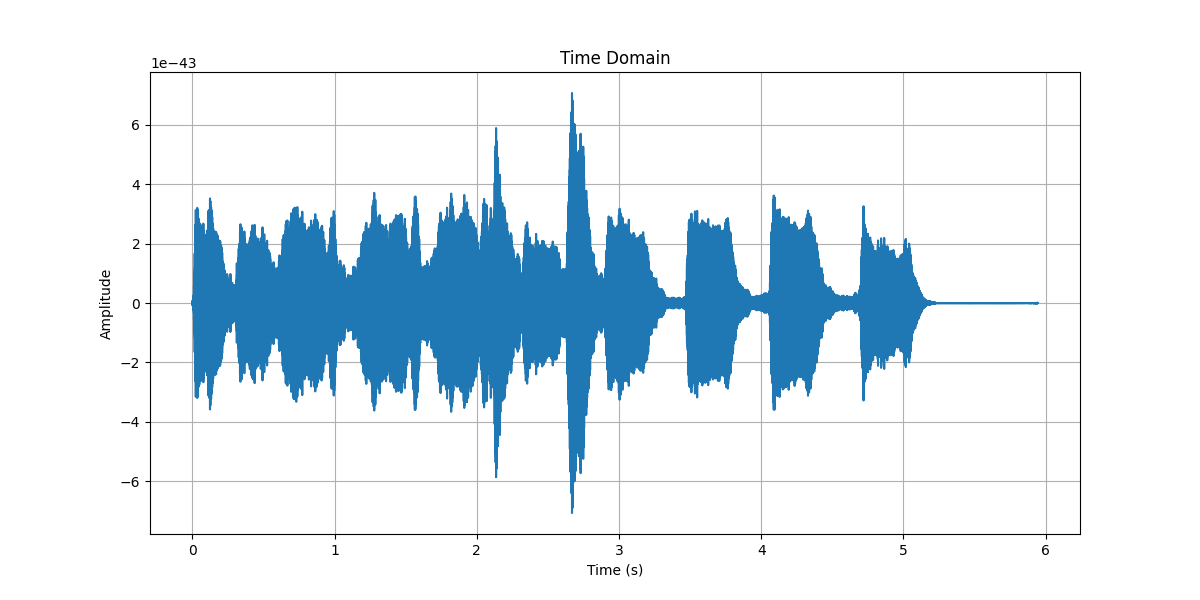
\includegraphics[width=1\textwidth]{high_pass_time_domain.png}
    \caption{High-pass filtered audio signal reversed to time domain}
    \label{fig:high_pass_filter_histogram}

\end{figure}

\subsection{Low-pass filtering}

\hspace{1 em}Low-pass filtering is a signal processing technique that allows low-frequency 
components of a signal to pass through while attenuating high-frequency components. In this 
section, we will implement a low-pass filter using the Fourier transform and apply it to the 
audio signal.

\begin{figure}[H]
    \centering
    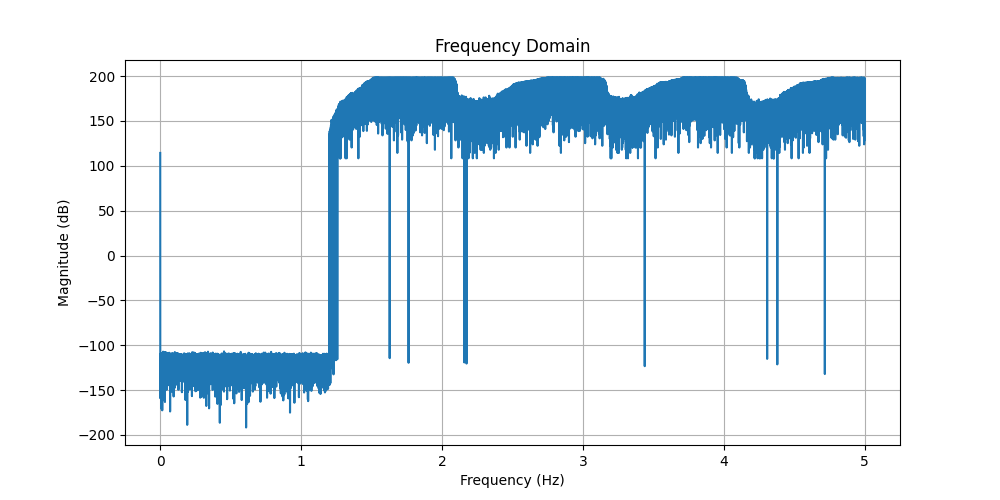
\includegraphics[width=1\textwidth]{low_pass_filter.png}
    \caption{Low-pass filtered audio signal}
    \label{fig:low_pass_filter}
\end{figure}

\begin{figure}[H]
    \centering
    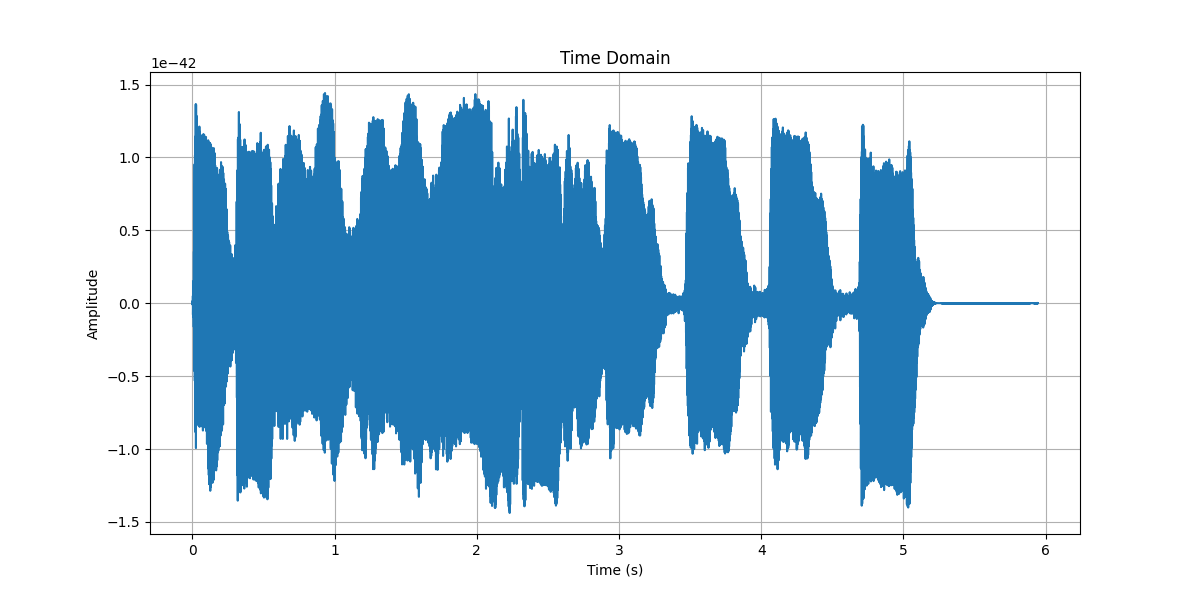
\includegraphics[width=1\textwidth]{low_pass_filter_time_domain.png}
    \caption{Low-pass filtered audio signal reversed to time domain}
    \label{fig:low_pass_filter_histogram}
\end{figure}

\newpage
\subsection{Mid-pass filtering}

\hspace{1 em}Mid-pass filtering is a signal processing technique that allows mid-frequency
components of a signal to pass through while attenuating low and high-frequency components.
In this section, we will implement a mid-pass filter using the Fourier transform and apply it
to the audio signal.

\begin{figure}[H]
    \centering
    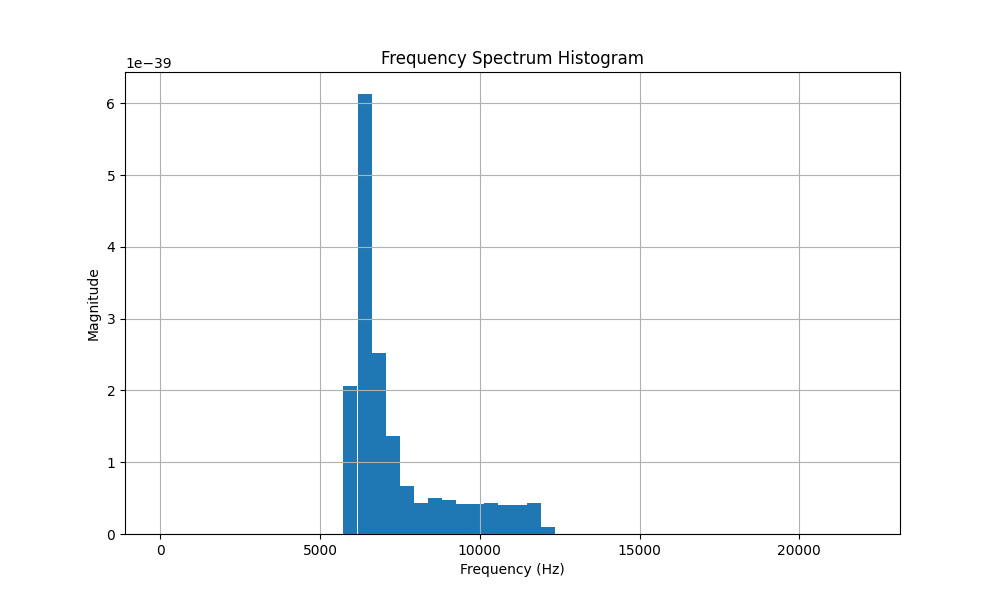
\includegraphics[width=1\textwidth]{mid_pass_filter.png}
    \caption{Mid-pass filtered audio signal}
    \label{fig:mid_pass_filter}
\end{figure}

\begin{figure}[H]
    \centering
    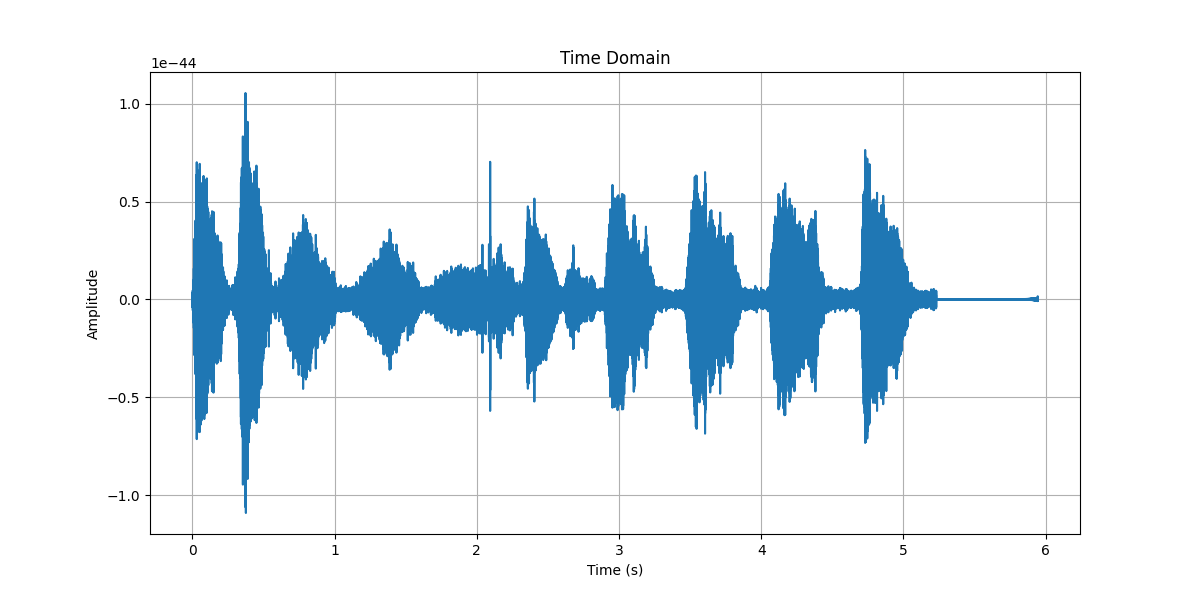
\includegraphics[width=1\textwidth]{mid_pass_filter_time.png}
    \caption{Mid-pass filtered audio signal reversed to time domain}
    \label{fig:mid_pass_filter_histogram}
\end{figure}

\newpage
\section{Additional signal examples}

\subsection{Example 1}

\begin{figure}[H]
    \centering
    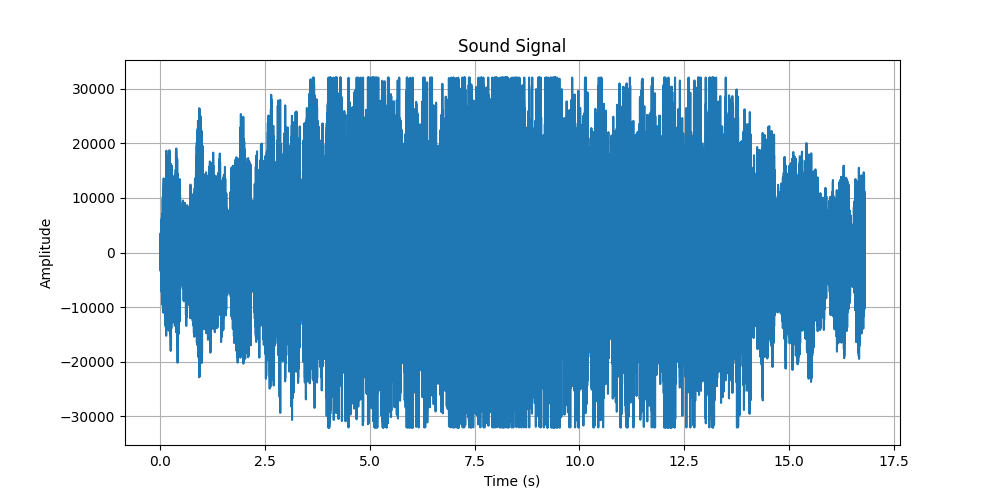
\includegraphics[width=1\textwidth]{ex2_raw.png}
    \caption{Unprocessed audio signal}
    \label{fig:ex2}
\end{figure}
\begin{figure}[H]
    \centering
    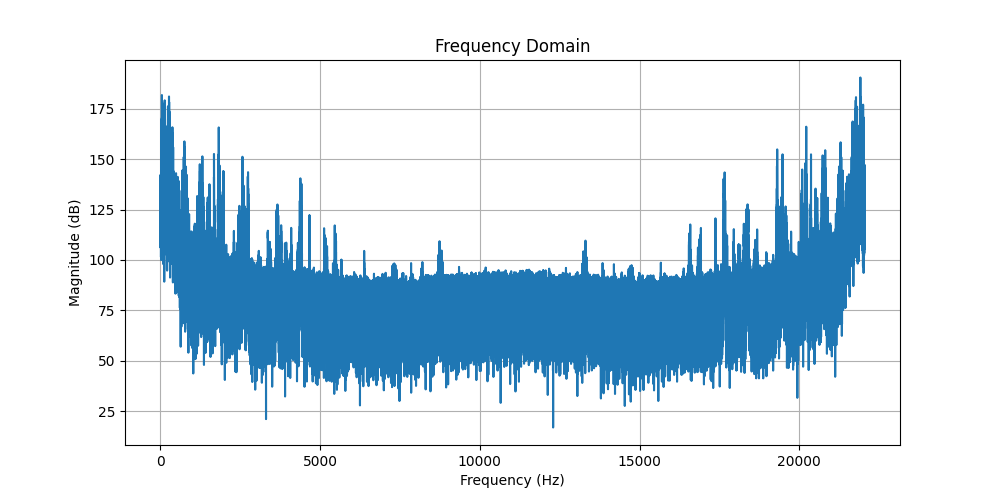
\includegraphics[width=1\textwidth]{ex2_frequency_domain.png}
    \caption{Power spectrum of the audio signal}
    \label{fig:ex2_freq}
    
\end{figure}
\begin{figure}[H]
    \centering
    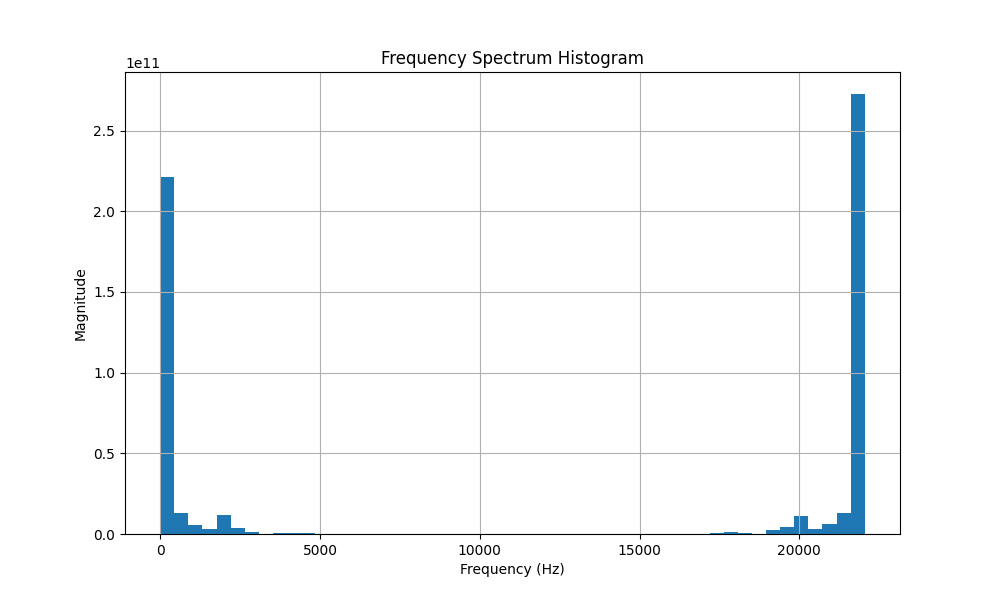
\includegraphics[width=1\textwidth]{ex2_spectrum_histogram.png}
    \caption{Signal in frequency domain and histogram}
    \label{fig:ex2_hist}
\end{figure}
\begin{figure}[H]
    \centering
    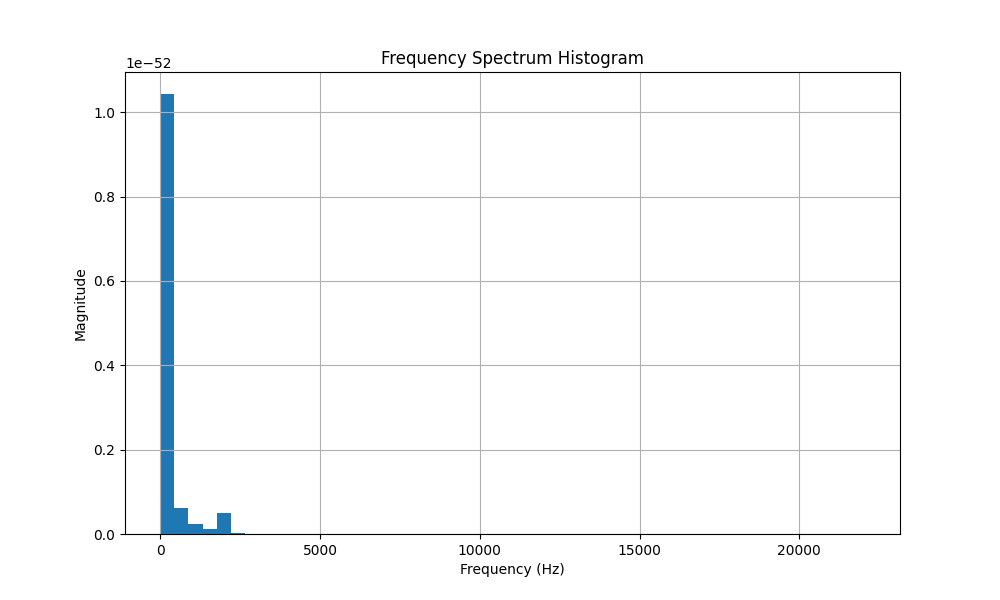
\includegraphics[width=1\textwidth]{ex2_low_pass_filter.png}
    \caption{Low-pass filtered audio signal}
    \label{fig:ex2_high}
\end{figure}
\begin{figure}[H]
    \centering
    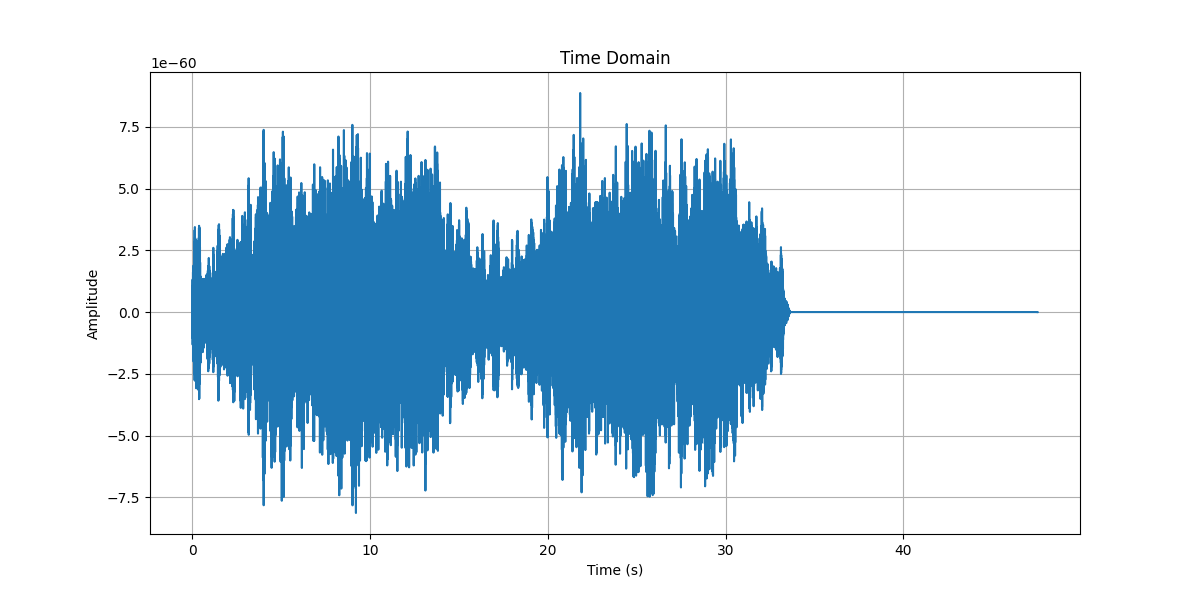
\includegraphics[width=1\textwidth]{ex2_low_pass_filter_time_domain.png}
    \caption{Low-pass filtered audio signal reversed to time domain}
    \label{fig:ex2_high_hist}
\end{figure}

\subsection{Example 2}

\begin{figure}[H]
    \centering
    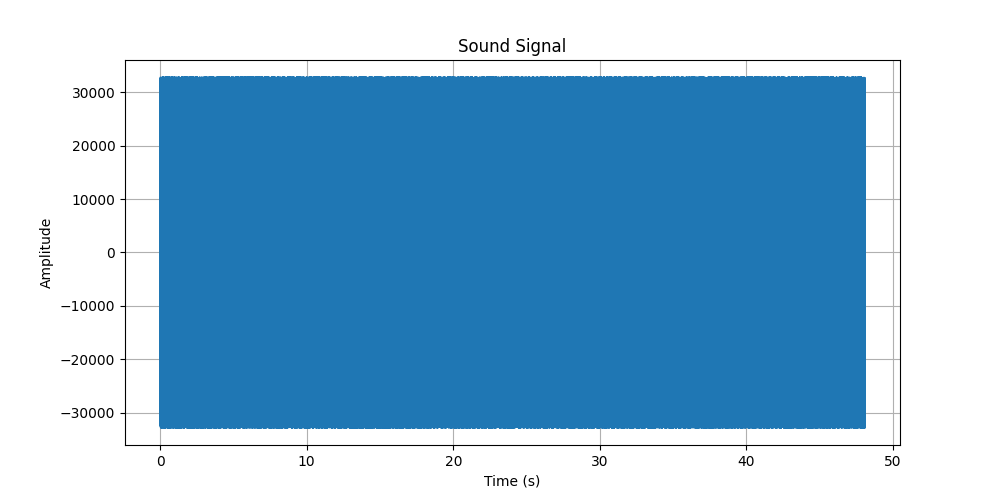
\includegraphics[width=1\textwidth]{ex3_raw.png}
    \caption{Unprocessed audio signal}
    \label{fig:ex3}
\end{figure}
\begin{figure}[H]
    \centering
    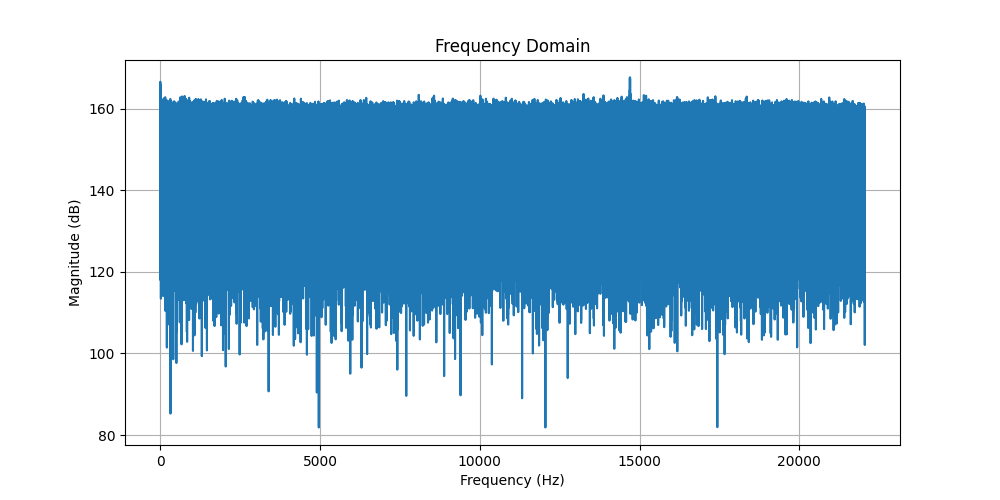
\includegraphics[width=1\textwidth]{ex3_frequency_domain.png}
    \caption{Power spectrum of the audio signal}
    \label{fig:ex3_freq}

\end{figure}

\begin{figure}[H]
    \centering
    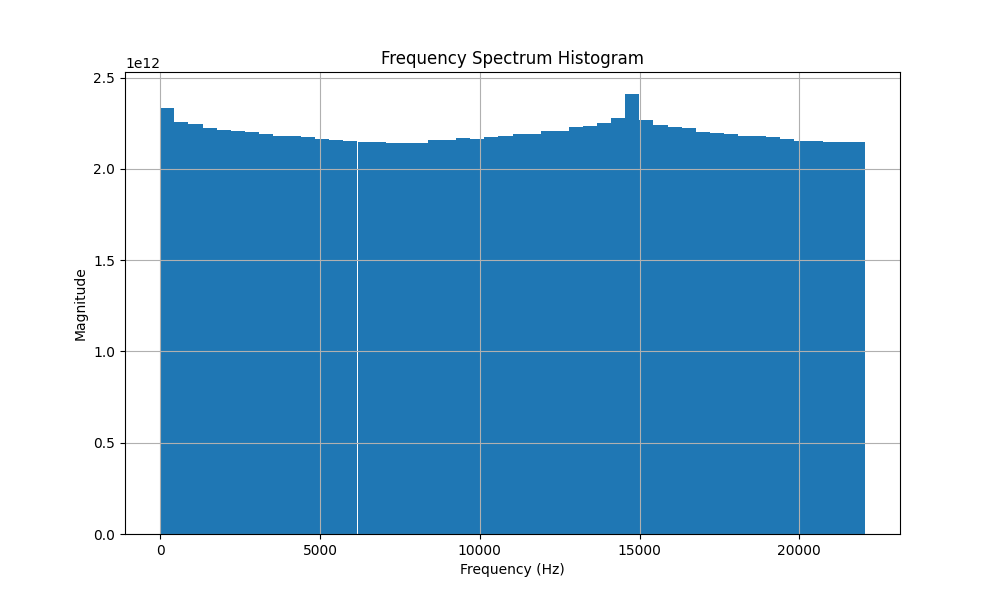
\includegraphics[width=1\textwidth]{ex3_spectrum_histogram.png}
    \caption{Signal in frequency domain and histogram}
    \label{fig:ex3_hist}
\end{figure}
\begin{figure}[H]
    \centering
    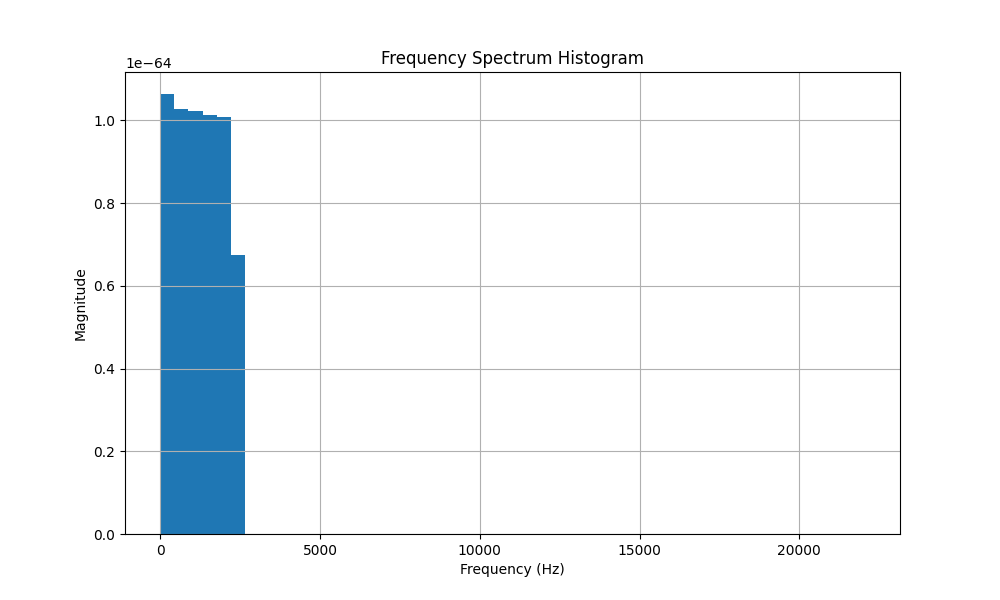
\includegraphics[width=1\textwidth]{ex3_low_pass_filter.png}
    \caption{Low-pass filtered audio signal}
    \label{fig:ex3_low}
\end{figure}
\begin{figure}[H]
    \centering
    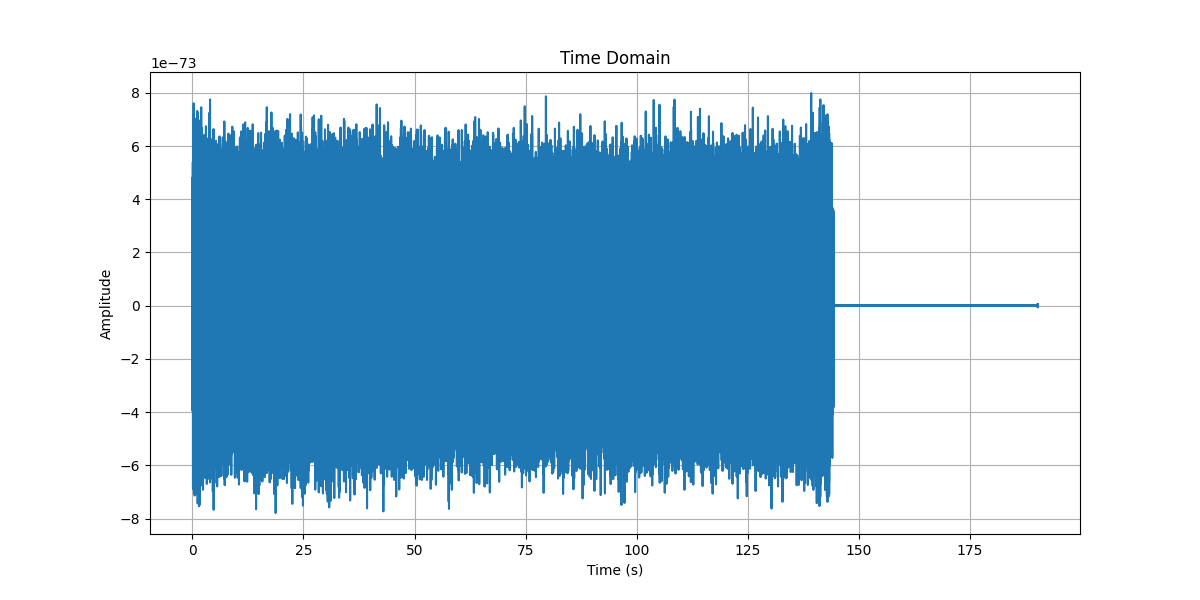
\includegraphics[width=1\textwidth]{ex3_low_pass_filter_time_domain.png}
    \caption{High-pass filtered audio signal reversed to time domain}
    \label{fig:ex3_low_hist}
\end{figure}

\subsection{Example 3}

\begin{figure}[H]
    \centering
    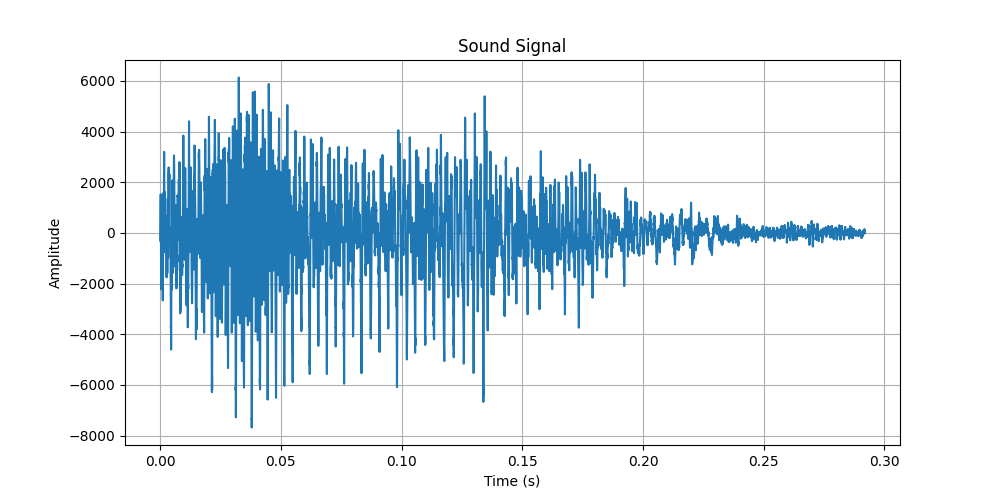
\includegraphics[width=1\textwidth]{ex4_raw.png}
    \caption{Unprocessed audio signal}
    \label{fig:ex4}
\end{figure}
\begin{figure}[H]
    \centering
    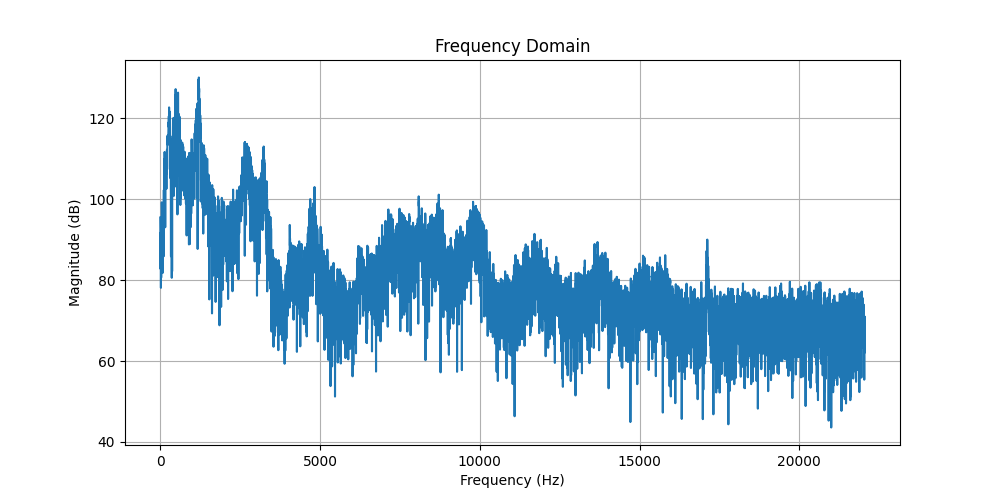
\includegraphics[width=1\textwidth]{ex4_frequency_domain.png}
    \caption{Power spectrum of the audio signal}
    \label{fig:ex4_freq}

\end{figure}

\begin{figure}[H]
    \centering
    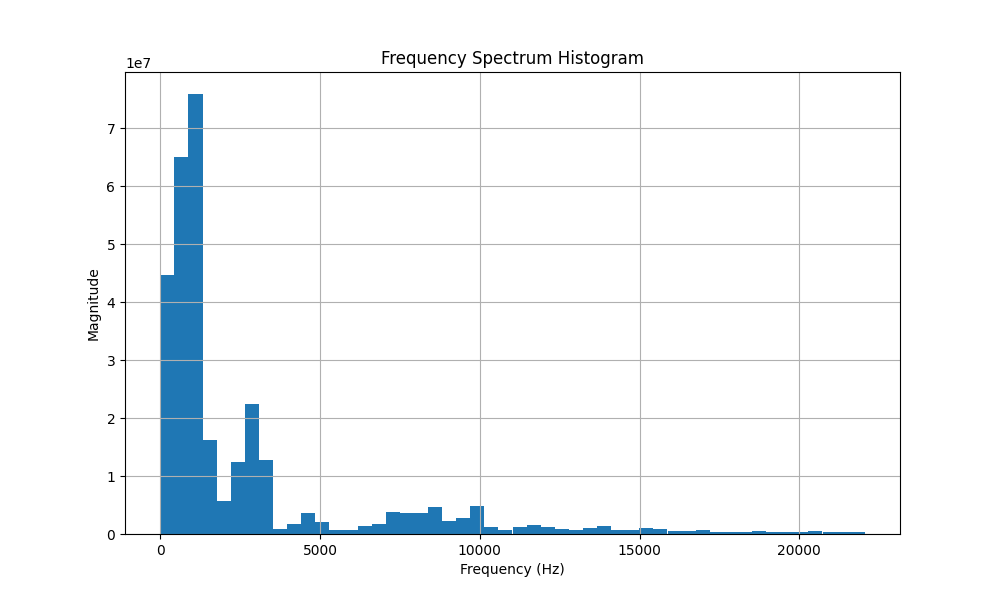
\includegraphics[width=1\textwidth]{ex4_spectrum_histogram.png}
    \caption{Signal in frequency domain and histogram}
    \label{fig:ex4_hist}
\end{figure}
\begin{figure}[H]
    \centering
    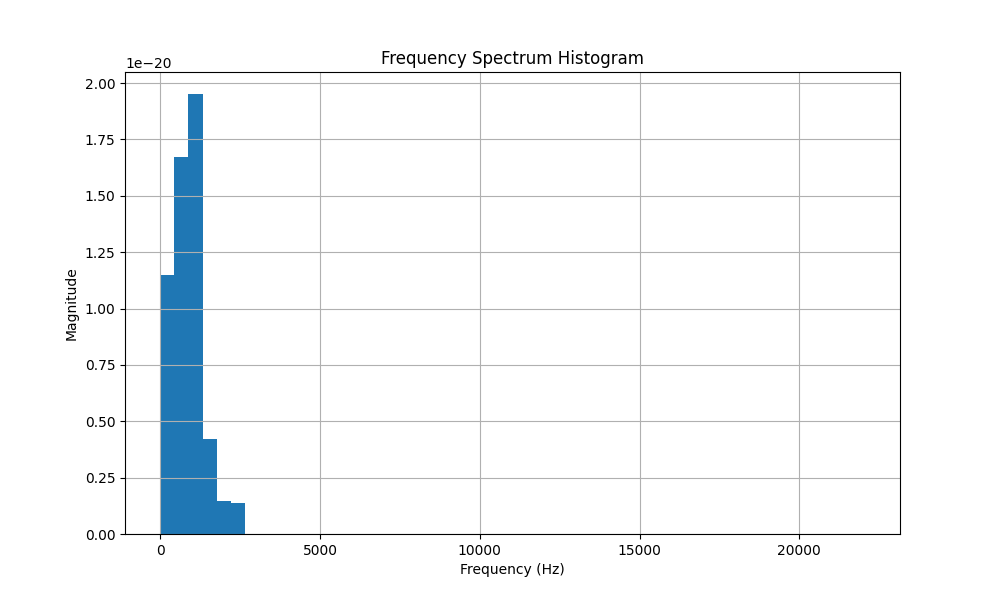
\includegraphics[width=1\textwidth]{ex4_low_pass_filter.png}
    \caption{Low-pass filtered audio signal}
    \label{fig:ex4_low}
\end{figure}
\begin{figure}[H]
    \centering
    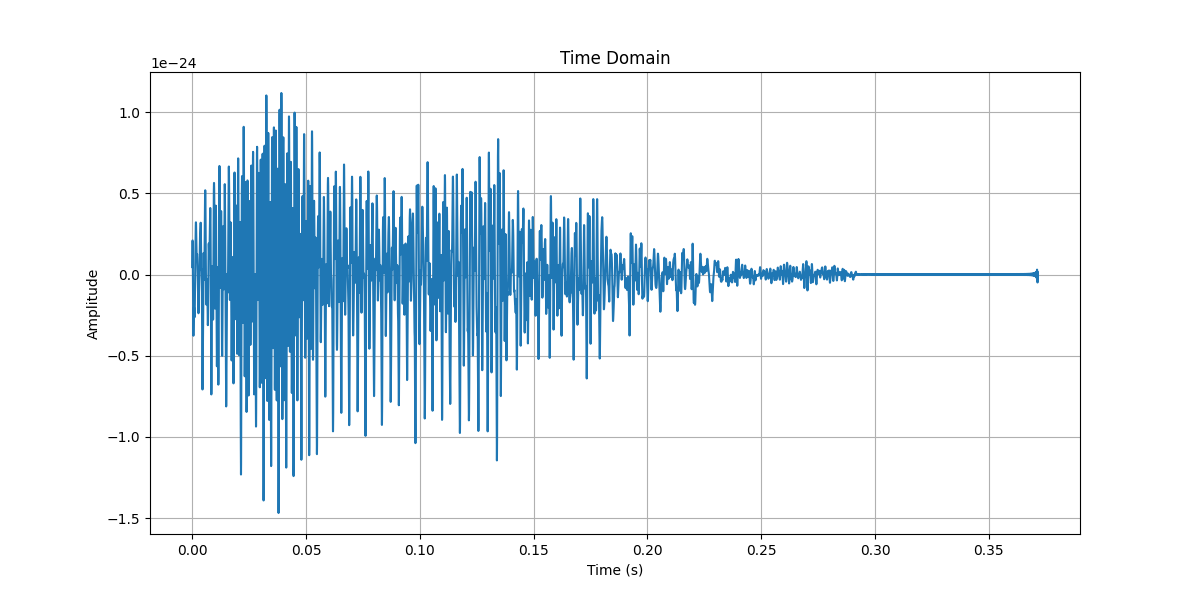
\includegraphics[width=1\textwidth]{ex4_low_pass_filter_time_domain.png}
    \caption{Low-pass filtered audio signal reversed to time domain}
    \label{fig:ex4_low_hist}
\end{figure}

\subsection{Example 4}

\begin{figure}[H]
    \centering
    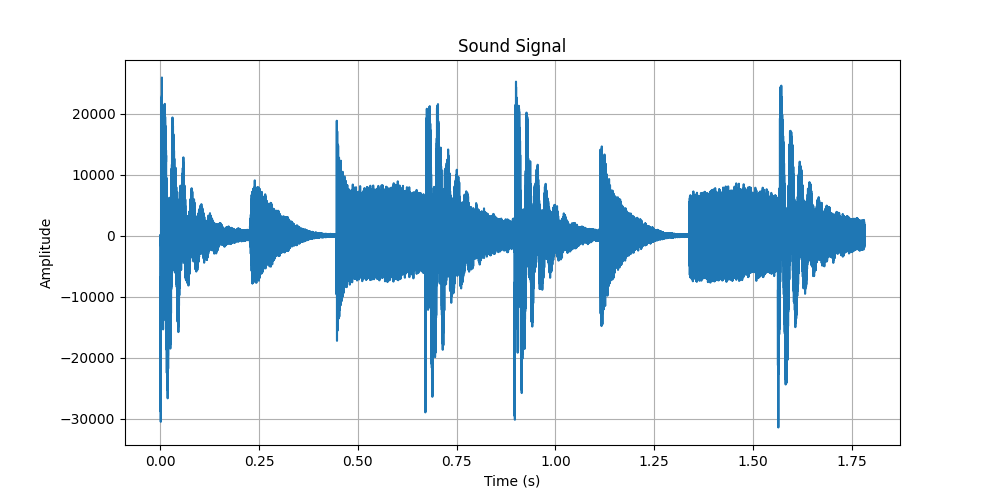
\includegraphics[width=1\textwidth]{ex5_raw.png}
    \caption{Unprocessed audio signal}
    \label{fig:ex5}
\end{figure}
\begin{figure}[H]
    \centering
    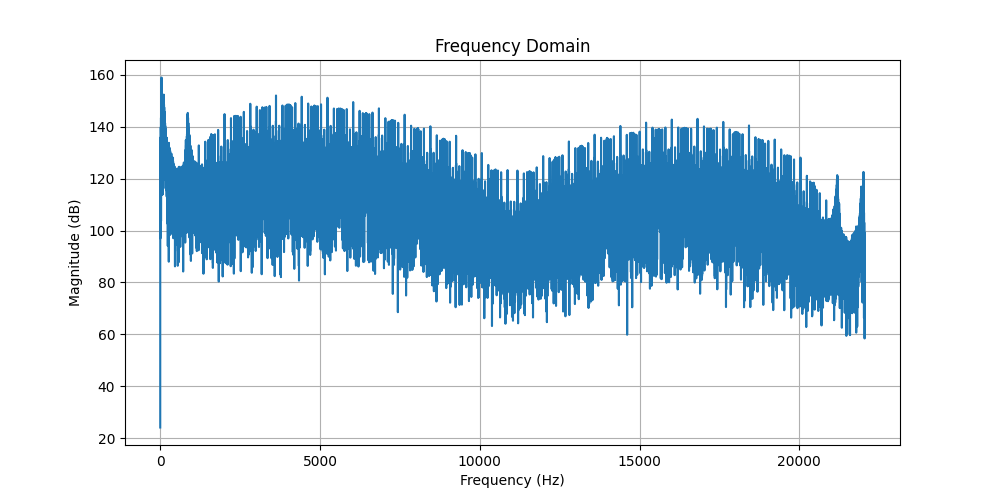
\includegraphics[width=1\textwidth]{ex5_frequency_domain.png}
    \caption{Power spectrum of the audio signal}
    \label{fig:ex5_freq}

\end{figure}

\begin{figure}[H]
    \centering
    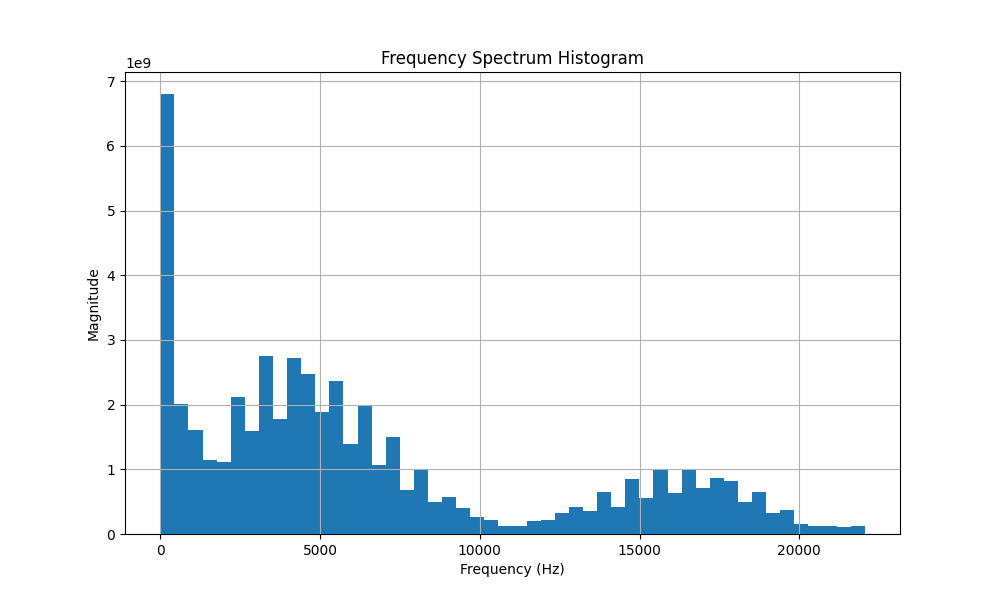
\includegraphics[width=1\textwidth]{ex5_spectrum_histogram.png}
    \caption{Signal in frequency domain and histogram}
    \label{fig:ex5_hist}
\end{figure}

\begin{figure}[H]
    \centering
    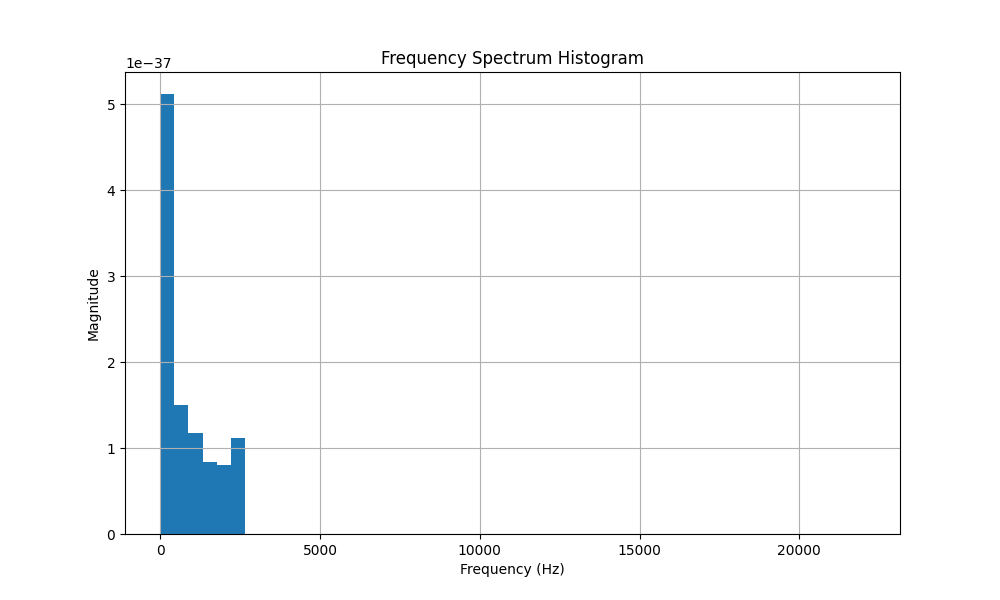
\includegraphics[width=1\textwidth]{ex5_low_pass_filter.png}
    \caption{Low-pass filtered audio signal}
    \label{fig:ex5_low}
\end{figure}
\begin{figure}[H]
    \centering
    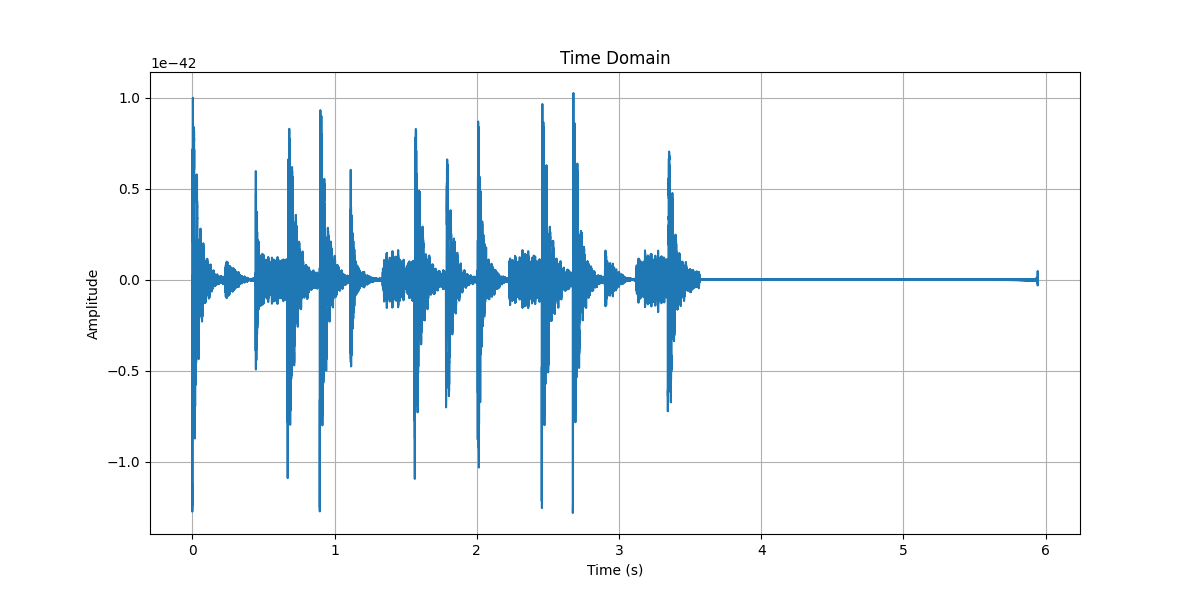
\includegraphics[width=1\textwidth]{ex5_low_pass_filter_time_domain.png}
    \caption{Low-pass filtered audio signal reversed to time domain}
    \label{fig:ex5_low_hist}
\end{figure}


\newpage

\section{Conclusion}

\hspace{1 em}In this report, we implemented the Discrete Fourier Transform (DFT), Fast Fourier Transform (FFT), Inverse Discrete Fourier Transform (IDFT), and Inverse Fast Fourier Transform (IFFT) algorithms from scratch. We compared the performance of the DFT and FFT algorithms and analyzed the impact of zero padding on the FFT algorithm's performance. We also implemented high-pass, low-pass, and mid-pass filters using the Fourier transform and applied them to audio signals to isolate specific frequency components. The results demonstrate the effectiveness of the Fourier filter in isolating and analyzing frequency components of audio signals.

On the other hand, the analysis of algorithm performance showed that implementation of FFT from scratch is suboptimal and needs to be improved. The comparison of FFT from scratch and numpy FFT showed that numpy FFT is significantly faster. The comparison of DFT and FFT showed that FFT is significantly faster than DFT. The comparison of FFT with and without zero padding showed that zero padding reduces the performance of the FFT algorithm.

FFT is a powerful algorithm that enables efficient analysis and processing of time domain signals and
their frequency components. By implementing and applying the FFT algorithm, we can gain insights into the frequency characteristics of signals and develop sophisticated signal processing techniques such as filtering, compression, and feature extraction.

\end{document}

